\documentclass[tikz,border=4pt]{standalone}
\usepackage{amsmath}
\begin{document}
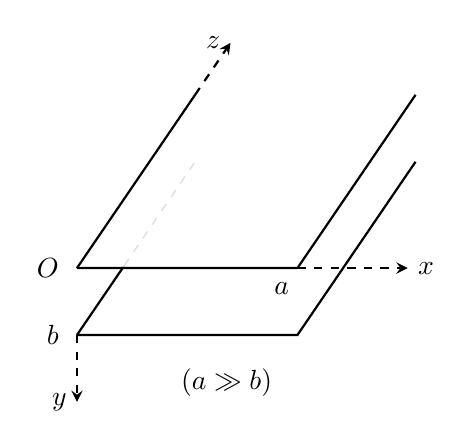
\begin{tikzpicture}[>=stealth, thick, scale=1.0]
  % Parallel plate transmission line:
  % O at (0,0), x goes right, y goes down, z goes up-right
  \coordinate (O) at (0, 0);
  \coordinate (A) at (2.8, 0);
  \coordinate (B) at (0, -0.85);
  \coordinate (AB) at (2.8, -0.85);
  \coordinate (Zvec) at (1.5, 2.2);

  % Lower plate
  \draw[thick] (B) -- (AB) -- ++(Zvec);
  \draw[thick] (B) -- ++(0.6, 0.88);
  \draw[dashed, thin] (0.6, 0.03) -- ++(0.9, 1.32);

  % Upper plate
  \fill[white, opacity=0.85] (O) -- (A) -- ++(Zvec) -- ++(-2.8, 0) -- cycle;
  \draw[thick] (O) -- (A) -- ++(Zvec);
  \draw[thick] (O) -- ++(Zvec);

  % Axes
  \draw[->, dashed, thick] (A) -- (4.2, 0) node[right] {$x$};
  \draw[->, dashed, thick] (B) -- (0, -1.7) node[left] {$y$};
  \draw[->, dashed, thick] (1.5, 2.2) -- (1.95, 2.86) node[left] {$z$};

  % Labels
  \node[left] at (-0.1, 0) {$O$};
  \node[below] at (2.6, -0.05) {$a$};
  \node[left] at (-0.1, -0.85) {$b$};
  \node at (1.9, -1.45) {$(a \gg b)$};
\end{tikzpicture}
\end{document}
